\section{Verification of \texorpdfstring{\cref{ass:one}}{Assumption}}\label{app:assumptions}

For the typical car ($d_f=0.9$, $d_w=2.6$, $d_b=0.8$, $w=1.8$, $\theta=35^\circ$, $m=0.18$, lengths in metres) the derived quantities are
\[
\begin{gathered}
  R=3.7132,\quad \Rm=2.8132,\quad \Rp=4.6132,\quad \rho=5.7906,\quad r=4.6820,\quad H=1.98,\\
  \varepsilon_b=0.0689,\quad \psi_{\rm fit}=0.04225,\quad \psi_d=0.03137,\quad \beta=0.17171,\quad \gamma=0.92175,\quad \psi_b=0.47852,
\end{gathered}
\]
and $\Lambda_1=5.83295$, $B_{\rm back}=8.200$.
Each inequality of \cref{ass:one} holds with a comfortable margin.
The tightest in relative terms is the first inequality of \ref{A:far}, $d_b\cos\psi_{\rm fit}-\Rp\sin\psi_{\rm fit}+\rho=6.395\ge\Lambda_1$ (a margin of $9.6\%$); next come the first inequality of \ref{A:min} ($5.059>3.588$), $B_{\rm back}\ge\Lambda_1$ and \ref{A:curbcase} ($3.947\ge2.702$).

We also checked \cref{ass:one} on the grid
\[
\begin{gathered}
  d_f\in\{0.6,0.8,1.0,1.2\},\quad d_w\in\{2.3,2.6,2.9,3.2\},\quad d_b\in\{0.5,0.7,0.9,1.1,1.3\},\\
  w\in\{1.6,1.75,1.9,2.05\},\quad \theta\in\{28^\circ,33^\circ,38^\circ,43^\circ\},
\end{gathered}
\]
always with $m=w/10$.
Of the $1280$ parameter sets, $1160$ satisfy $m\ge\varepsilon_b$, and $1129$ of those satisfy all of \ref{A:db}--\ref{A:far}.
The $31$ exceptions are short and very wide cars ($d_w=2.3$ together with $w\ge1.9$, mostly with $d_f=0.6$, or with $\theta=43^\circ$).
For these either $B_{\rm back}\ge\Lambda_1$ fails ($21$ sets) or the condition $H<\Rm+d_b$ of \ref{A:fit} fails ($12$ sets, two of them also in the first group); they are far from real passenger cars.
The check is a short script, \texttt{numerics/assumptions.py} in the accompanying repository.
It evaluates the inequalities as stated, except that it also requires $Hb>\ell h_0$, so that $\log^+=\log$ in \eqref{eq:Bback}; this conservative extra condition changes none of the counts.

\section{Other car configurations}\label{app:cars}

\Cref{tab:cars} lists slot lengths for six cars, from a small city car to a large van, always with margin $m=w/10$.
The third row is the typical car of \cref{tab:values}.
For every car we checked \cref{ass:one} with the script described in \cref{app:assumptions}, and all seven groups of inequalities hold, so the column $n=1$ is exact.

For the first three cars the hypotheses of \cref{prop:two-better} hold, and the two-manoeuvre exit was also confirmed by an exact simulation.
For the three larger cars the triple-contact equations \eqref{eq:tc1}--\eqref{eq:tc2} have their solution at $\alpha_1<\beta$, outside the range of the proposition.
Their two-manoeuvre entries come from the numerical search of \cref{app:numerics}, restricted to two manoeuvres.
The columns $n=3,4,5$ come from the same search, started from the optimal parameters of the typical car.
Every reported value was confirmed by simulating the complete exit (script \texttt{numerics/car\_table.py}).

\begin{table}[ht]
\centering\small
\setlength{\tabcolsep}{4pt}
\begin{tabular}{@{}l*{5}{c}cc*{5}{c}c@{}}
\toprule
& $d_f$ & $d_w$ & $d_b$ & $w$ & $\theta$ & $\ell$ & $R$ & $n=1$ & $n=2$ & $n=3$ & $n=4$ & $n=5$ & $K$\\
\midrule
City car & 0.65 & 2.35 & 0.55 & 1.65 & $37^\circ$ & 3.55 & 3.12 & 4.910 & 4.517 & 4.311 & 4.222 & 4.132 & 4.51\\
Compact & 0.85 & 2.60 & 0.75 & 1.78 & $36^\circ$ & 4.20 & 3.58 & 5.686 & 5.271 & 5.126 & 5.024 & 4.911 & 5.02\\
Typical & 0.90 & 2.60 & 0.80 & 1.80 & $35^\circ$ & 4.30 & 3.71 & 5.833 & 5.411 & 5.280 & 5.180 & 5.050 & 5.15\\
Mid-size sedan & 0.95 & 2.85 & 1.00 & 1.84 & $34^\circ$ & 4.80 & 4.23 & 6.452 & 6.052$^{*}$ & 5.926 & 5.844 & 5.744 & 5.55\\
Large SUV & 1.00 & 3.00 & 1.05 & 1.98 & $33^\circ$ & 5.05 & 4.62 & 6.877 & 6.393$^{*}$ & 6.288 & 6.187 & 6.069 & 6.03\\
Van & 1.00 & 3.40 & 1.10 & 2.00 & $31^\circ$ & 5.50 & 5.66 & 7.543 & 6.969$^{*}$ & 6.850 & 6.734 & 6.597 & 6.71\\
\bottomrule
\end{tabular}
\caption{Slot lengths (in metres) for parallel parking with $n$ manoeuvres, for six car configurations with margin $m=w/10$.
The column $n=1$ is the exact value $\Lmin(1)=\Lambda_1$ of \cref{thm:one}.
The column $n=2$ is $\Lambda_2^*$ from \cref{prop:two-better}; entries marked $^*$ are numerical, because there the double contact occurs before the rear corner passes the bottom of its circle ($\alpha_1<\beta$, cf.\ \cref{rem:two-other}).
The columns $n=3,4,5$ are the best rotation zigzags found.
All entries with $n\ge2$ are upper bounds for $\Lmin(n)$.
For large $n$, $\Lmin(n)=\ell+K/\sqrt n+o(n^{-1/2})$ by \cref{thm:asym}.}
\label{tab:cars}
\end{table}


Some trends are visible.
\begin{itemize}[nosep]
\item The extra length over the car, $\Lmin(1)-\ell$, grows from $1.36$ m for the city car to $2.04$ m for the van, mainly through the turning radius $R$, which enters $\Lambda_1$ through the term $\sqrt{\rho^2-(r-H)^2}$.
\item A second manoeuvre saves $0.39$--$0.57$ m, and five manoeuvres save $0.71$--$0.95$ m compared with one.
\item The classical formula $d_b+\sqrt{b^2+2Rw}$ overestimates $\Lmin(1)$ by $0.02$--$0.04$ m for all six cars.
\item The constant $K$ ranges from $4.5$ to $6.7$ m. For a small slack $g=L-\ell$ about $K^2/g^2\approx4Rw/g^2$ manoeuvres are needed, so this number is roughly proportional to the turning radius times the width.
\end{itemize}

\section{A five-manoeuvre parking motion}\label{app:five}

\Cref{fig:five} shows the best five-manoeuvre motion we found for the typical car, in the slot $L=5.050$~m of \cref{tab:zigzag} (more precisely $5.0497$~m).
This slot is only $0.75$ m longer than the car and $0.78$ m shorter than the one-manoeuvre slot $\Lmin(1)=5.833$ m.
For five manoeuvres the rotation zigzag of \cref{sec:zigzag} is far better than the crawl of \cref{sec:asym}, which in our simulations needs $28$ manoeuvres already for $L=5.3$ m (\cref{fig:values}).
The motion is drawn in forward (parking) time; it is the time reversal of the optimised exit (\cref{lem:reversal}).
In driving terms:
\begin{enumerate}[nosep]
\item reverse into the slot along an S-curve, first with full right lock and then with full left lock, until the rear curb-side corner touches the curb; the car now points $0.40$ rad ($23^\circ$) nose-up;
\item pull forward $0.16$ m with full right lock until the front curb-side corner touches the bumper of the car in front (tilt $0.36$ rad);
\item reverse $0.50$ m with full left lock until the rear corners touch the curb and the bumper of the car behind (tilt $0.22$ rad);
\item pull forward $0.47$ m, with full right lock and for the last $0.14$ m with full left lock, stopping $3$ mm short of the car in front (tilt $0.17$ rad);
\item reverse $0.65$ m with full left lock into the level parked position, against the car behind.
\end{enumerate}
Each manoeuvre turns the car further towards level.
There is no sideways slip: the rear wheels roll along their paths, which are tangent to them at every instant, while the overhangs behind the rear axle and in front of it swing sideways as the car turns.
The contacts show what limits each step: the curb and the car behind limit the reverse manoeuvres, and the car in front limits the forward ones.
The motion was checked with the exact collision test of \cref{app:numerics} (script \texttt{numerics/fig\_five.py}).

\begin{figure}[ht]
\centering
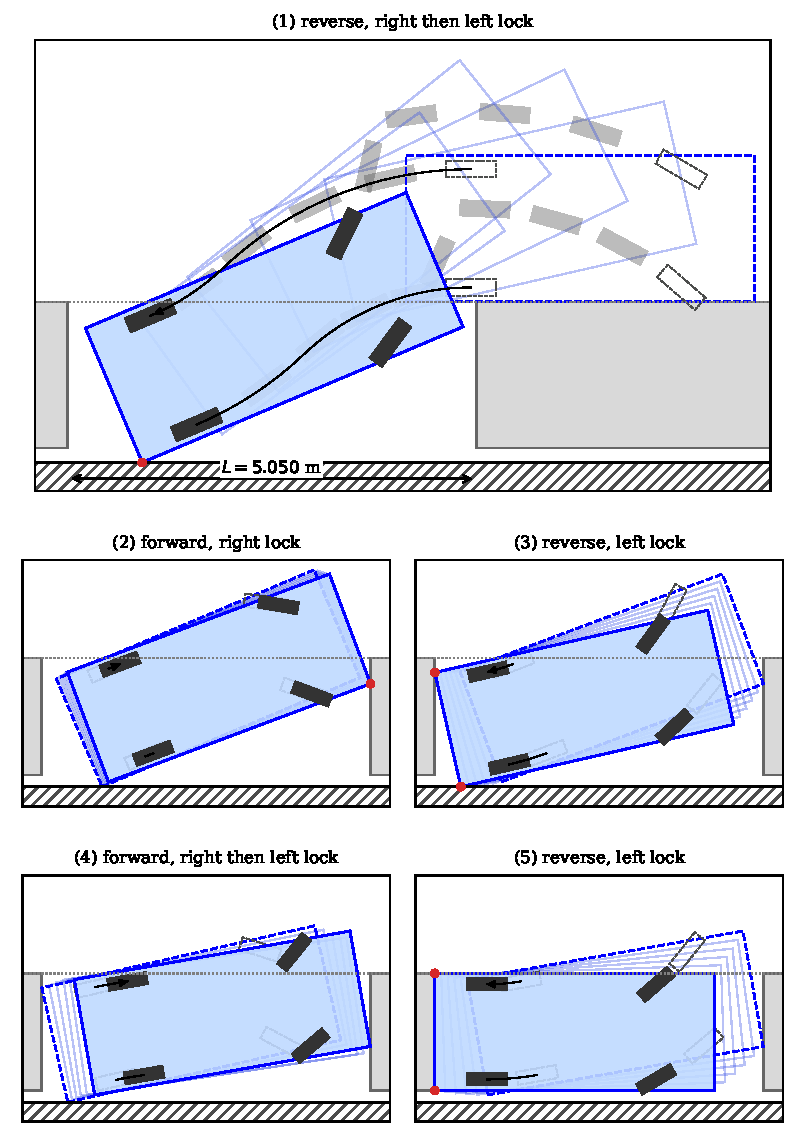
\includegraphics[width=\textwidth,height=0.8\textheight,keepaspectratio]{figures/fig_five.pdf}
\caption{The best five-manoeuvre parking motion found for the typical car, in a slot of length $L=5.050$ m.
Each panel shows one manoeuvre: start (dashed), intermediate positions (thin), end (filled), the paths of the two rear wheels with the direction of travel (black), and the contacts at the end of the manoeuvre (red dots).
The front wheels are drawn at the Ackermann angles of full lock.
Panel (1) is drawn at a smaller scale and also shows the wheels at the intermediate positions.}
\label{fig:five}
\end{figure}
\clearpage

\section{A twenty-manoeuvre parking motion}\label{app:twenty}

\Cref{fig:twenty} shows the same car parking with $20$ manoeuvres in a slot of length $L=4.855$ m.
This slot is $0.555$ m longer than the car, $0.195$ m shorter than the five-manoeuvre slot of \cref{fig:five}, and $0.98$ m shorter than $\Lmin(1)$.
We found it by searching \emph{contact zigzags}, which we describe as exits (the time reversals of parking motions).
Every full-lock arc is driven until the car touches the curb or a parked car, except for an optional left-lock arc of a fixed angle $a\in\{0,0.02,\dots,0.08\}$ rad before each reverse arc; the escape is tried before every manoeuvre.
The parked starting position, the direction of the first exit manoeuvre and $a$ were searched on a grid, which was then refined near the optimum, and bisection on $L$ located the shortest slot.
The best exit found has $a=0$.
Every manoeuvre was checked with the exact collision test (scripts \texttt{numerics/twenty\_search.py} and \texttt{numerics/fig\_twenty.py}).
The value is therefore an upper bound for $\Lmin(20)$.

The motion has three phases.
\begin{enumerate}[nosep]
\item The car reverses into the slot along an S-curve ($4.04$ m) and ends tilted by $26.7^\circ$, with its rear curb-side corner on the curb.
\item In manoeuvres 2--16 it is wedged between the curb and the car in front.
It alternately pulls forward with full right lock until its front curb-side corner touches the car in front, and reverses with full left lock until its rear curb-side corner touches the curb.
Each of these manoeuvres is only $2$--$10$ cm long and turns the car by $0.3^\circ$--$1.5^\circ$.
\item As the tilt decreases the wedge opens, and the steps grow: manoeuvres 17--20 are $19$--$41$ cm long and bring the car from $17.6^\circ$ to level. The reverse manoeuvres now end when the rear bumper touches the car behind, and the last forward manoeuvre ends in the level parked position.
\end{enumerate}
The number of manoeuvres needed grows very quickly as the slot shrinks.
In our searches $14$ manoeuvres suffice for $L=4.888$ m and $20$ for $L=4.855$ m, while for $L=4.80$ m the zigzag stalls: the rotation gained per manoeuvre tends to zero.
For comparison, the lateral crawl of \cref{sec:asym} needs $69$ manoeuvres for $L=4.9$ m and $97$ for $L=4.8$ m in our simulations (\cref{fig:values}); below about $4.85$ m it is the only strategy we know.
Accordingly, the asymptotic formula $\ell+K/\sqrt{n}$, which equals $5.45$ m for $n=20$, describes $\Lmin(n)$ only for much larger $n$.

\begin{figure}[p]
\centering
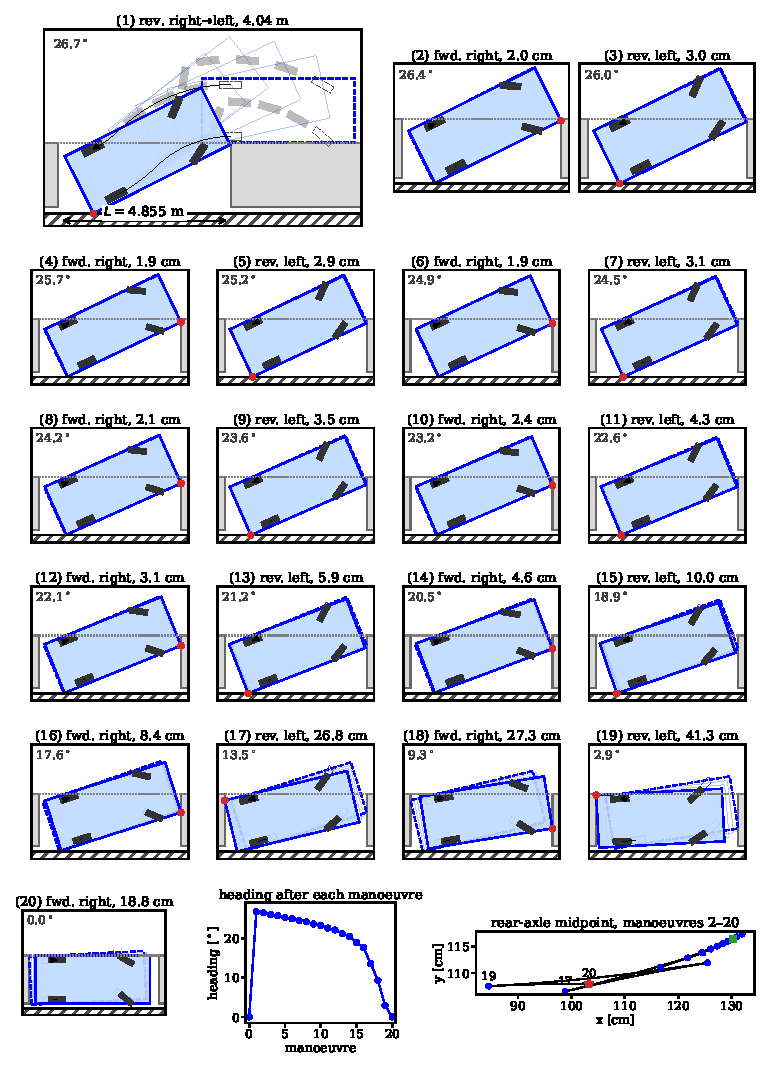
\includegraphics[width=\textwidth,height=0.84\textheight,keepaspectratio]{figures/fig_twenty.pdf}
\caption{The best twenty-manoeuvre parking motion found for the typical car, in a slot of length $L=4.855$ m.
Each panel shows one manoeuvre, drawn as in \cref{fig:five}: start (dashed), end (filled), wheels, rear-wheel paths, and contacts at the end (red dots).
The title gives the direction (fwd./rev.), the steering (full left or right lock) and the distance driven; the number in the corner is the heading at the end.
Panel (1) is drawn at a smaller scale.
Bottom: the heading after each manoeuvre, and the path of the rear-axle midpoint during manoeuvres 2--20 (green square: after manoeuvre 1; red star: parked).}
\label{fig:twenty}
\end{figure}
\clearpage

\section{A five-manoeuvre parking motion with a soft curb}\label{app:five-soft}

\Cref{fig:five-soft} shows the best five-manoeuvre motion we found for the typical car with a soft curb (\cref{sec:model-soft,sec:soft}), in a slot of length $L=4.906$~m (more precisely $4.9051$~m).
This is $0.14$ m less than the rigid-curb slot of \cref{fig:five}, only $0.61$ m longer than the car, and $0.90$ m shorter than the one-manoeuvre slot $\Lmins(1)=5.809$ m.
In driving terms:
\begin{enumerate}[nosep]
\item reverse into the slot along an S-curve, first with full right lock and then with full left lock, until the rear bumper touches the car behind; the car now points $0.38$ rad ($22^\circ$) nose-up, and its rear overhang passes up to $7.1$ cm beyond the curb;
\item pull forward $0.24$ m with full right lock until the front curb-side corner touches the car in front (tilt $0.32$ rad);
\item reverse $0.33$ m with full left lock until the rear bumper touches the car behind (tilt $0.23$ rad);
\item pull forward $0.34$ m with full right lock until the front curb-side corner touches the car in front (tilt $0.14$ rad);
\item reverse $0.52$ m with full left lock into the level parked position, against the car behind.
\end{enumerate}
The difference from \cref{fig:five} is that the curb no longer stops the reverse manoeuvres.
Each manoeuvre is a single full-lock arc driven until the car touches a parked car, so the car shuffles between the two parked cars; in the terminology of \cref{app:twenty} the motion is a contact zigzag with $a=0$.
The tyres stay at least $14.8$ cm from the curb.
We found the motion with the full search of \cref{app:numerics}.
All its parameters ended at their bounds, so the motion is determined by $L$, and we located the shortest slot by bisection on $L$.
The motion was checked with the exact collision test, also with the front tyres turned to the Ackermann angles and with the largest tyres of \cref{sec:compare} (scripts \texttt{numerics/fig\_five.py} with the argument \texttt{soft}, and \texttt{numerics/soft\_checks.py}).

\begin{figure}[ht]
\centering
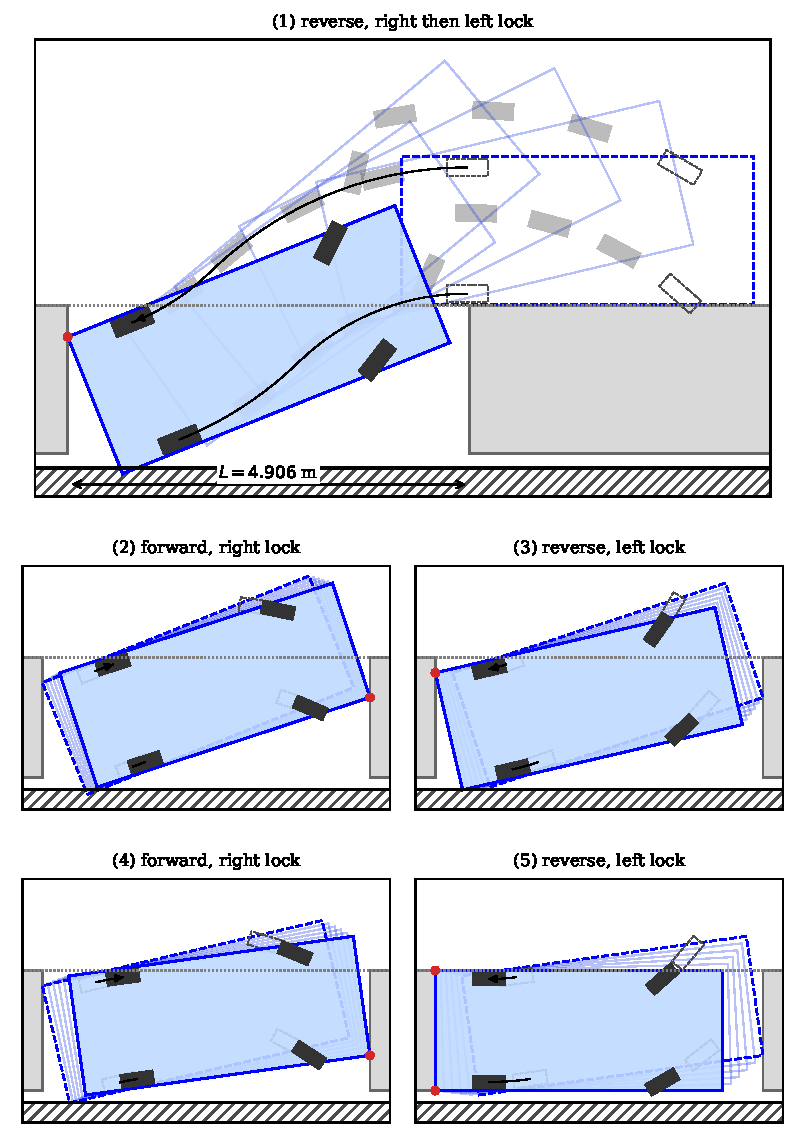
\includegraphics[width=\textwidth,height=0.8\textheight,keepaspectratio]{figures/fig_five_soft.pdf}
\caption{The best five-manoeuvre parking motion found for the typical car with a soft curb, in a slot of length $L=4.906$ m, drawn as in \cref{fig:five}.
The tyres are drawn with the data of \cref{sec:model-soft}, the front tyres at the Ackermann angles of full lock.
The bodywork may pass over the curb (hatched); the tyres may not.}
\label{fig:five-soft}
\end{figure}
\clearpage

\section{A twenty-manoeuvre parking motion with a soft curb}\label{app:twenty-soft}

\Cref{fig:twenty-soft} shows the typical car parking with $20$ manoeuvres and a soft curb, in a slot of length $L=4.704$ m (more precisely $4.7032$ m).
This is $0.15$ m less than with a rigid curb (\cref{fig:twenty}), $0.40$ m longer than the car, and $0.20$ m shorter than the soft-curb five-manoeuvre slot of \cref{fig:five-soft}.
We found it with the contact-zigzag search of \cref{app:twenty}, using the soft-curb collision test.
The best exit found starts from the parked position against the car in front, begins with a reverse manoeuvre and has $a=0$.
In parking time the car therefore ends with a forward manoeuvre against the car in front.
The motion has two phases.
\begin{enumerate}[nosep]
\item The car reverses into the slot along an S-curve ($4.10$ m) and ends tilted by $26.6^\circ$, with its rear bumper against the car behind; its rear overhang passes $5.2$ cm beyond the curb.
\item In manoeuvres 2--20 it is wedged between the two parked cars.
It alternately pulls forward with full right lock until its front curb-side corner touches the car in front, and reverses with full left lock until its rear bumper touches the car behind.
The steps grow as the tilt decreases.
Manoeuvres 2--12 are $4$--$6$ cm long and turn the car by $0.6^\circ$--$0.9^\circ$ each.
Manoeuvres 17--20 are $14$--$33$ cm long and bring the car from $13.1^\circ$ to level; the last one ends in the level parked position.
\end{enumerate}
Unlike the rigid-curb motion, this motion has no phase in which the car is wedged against the curb.
Its tyres stay at least $16$ cm from the curb, and from manoeuvre 15 on the whole body is above the curb line.
The motion was checked as in \cref{app:five-soft} (scripts \texttt{numerics/twenty\_search.py} and \texttt{numerics/fig\_twenty.py} with the argument \texttt{soft}).
The value is therefore an upper bound for $\Lmins(20)$.

\begin{figure}[p]
\centering
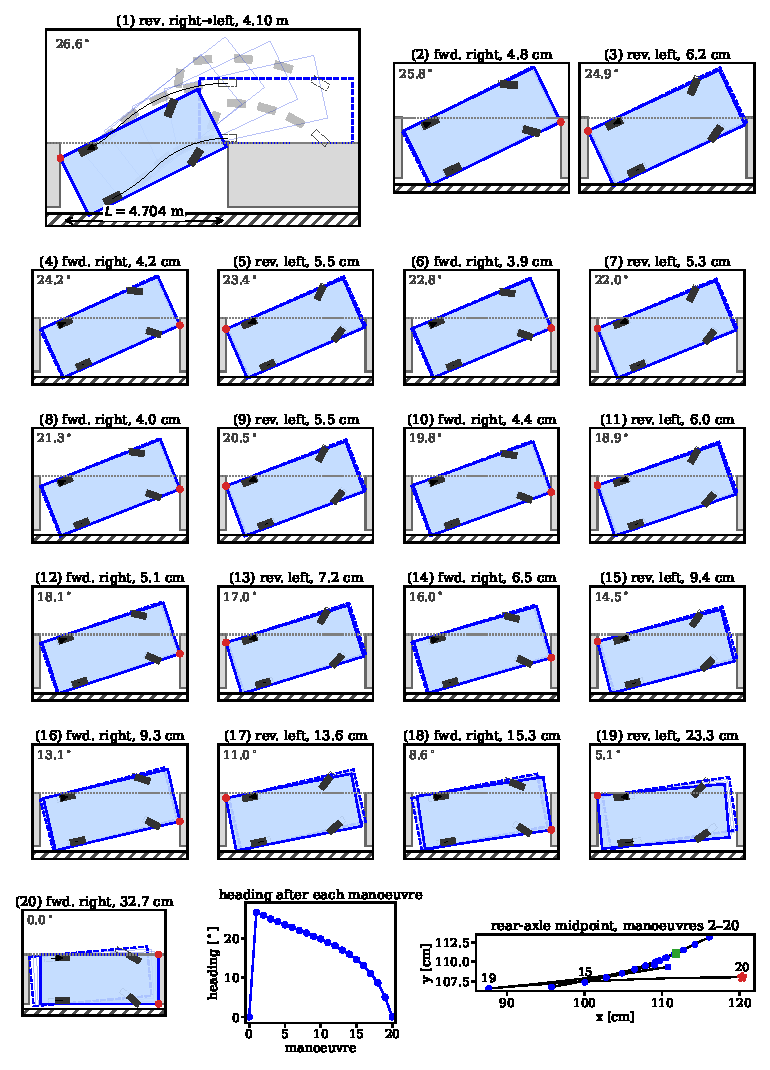
\includegraphics[width=\textwidth,height=0.84\textheight,keepaspectratio]{figures/fig_twenty_soft.pdf}
\caption{The best twenty-manoeuvre parking motion found for the typical car with a soft curb, in a slot of length $L=4.704$ m, drawn as in \cref{fig:twenty}, with the tyres of \cref{sec:model-soft}.
Panel (1) is drawn at a smaller scale.
Bottom: the heading after each manoeuvre, and the path of the rear-axle midpoint during manoeuvres 2--20 (green square: after manoeuvre 1; red star: parked).}
\label{fig:twenty-soft}
\end{figure}
\clearpage

\section{Numerical methods}\label{app:numerics}

\paragraph{Collision test.}
A configuration is tested exactly: each edge of the footprint is clipped against the open strips $\Or$, $\Of$, and the lowest corner is compared with the curb.
In the searches the configuration is sampled along each arc with step $2$--$3$ mm, and contact times are refined by bisection to $10^{-9}$ m; the figure scripts re-check each motion with $400$ samples per arc.
For the soft curb the lowest corner is replaced by the lowest corner of the tyre rectangles.

\paragraph{Strategy search.}
For $n\le6$ we parametrised exits by the starting position (level, at the top of the slot) and, for each manoeuvre, the fraction of the maximal collision-free length of its full-right-lock or forward full-left-lock arc, together with the angle (at most $0.1$ rad) of the optional left-lock arc of a reverse manoeuvre.
Forward manoeuvres were single full-left-lock arcs.
Reverse manoeuvres were either a single full-right-lock arc or a short full-left-lock arc followed by a full-right-lock arc.
For each trial length $L$ the parameters were optimised by differential evolution (with polishing) so as to maximise $L-V$ at the end; feasibility was then confirmed by simulating the final exit.
The minimal feasible $L$ was located by bisection.
The values are upper bounds for $\Lmin(n)$ and are rounded up to three decimals.
For \cref{tab:cars,tab:compare} a lighter version was used: $40$ generations without polishing, warm-started from the optimal parameters of the typical car, and stopped as soon as a verified exit was found.
For the typical car it reproduced the values for $n=3$ and $5$ and improved the value for $n=4$ from $5.184$ to $5.180$ m.
With a soft curb the light search gave $4.140$ m for the city car with five manoeuvres, more than the rigid-curb value $4.132$ m.
We therefore ran a second pass for this entry, warm-started from the car's own rigid-curb zigzag.
A rigid-curb motion is also free with a soft curb, so this pass can only improve a value; it gave $4.128$ m.
For the typical car the soft-curb values with $n=3,4,5$ come from the full search, as the rigid-curb values of \cref{tab:zigzag}.
It gave $5.088$, $4.978$ and $4.906$ m, against $5.089$, $4.988$ and $4.923$ m from the light search, which can therefore miss the best zigzag by up to $2$ cm.
In all three cases the optimal parameters lie at their bounds, so the motion is a contact zigzag in the sense of \cref{app:twenty}, determined by $L$; we then located the shortest slot by bisection on $L$.

\paragraph{Checks of the soft-curb motions.}
The script \texttt{numerics/soft\_checks.py} re-simulates the soft-curb motions behind \cref{tab:compare} and behind the soft-curb twenty-manoeuvre value with $400$ samples per arc, in three tyre models.
These are the model of \cref{sec:model-soft}, the same model with the front tyres turned to the Ackermann angles of the current full-lock arc, and, for $n\ge2$, the model with the largest tyres of \cref{sec:compare} ($\delta_s=0$, $\lambda=0.30$ m).
All motions are free in all three.
The script also reports the clearances quoted in \cref{sec:soft,sec:compare}.

\paragraph{Crawls.}
For \cref{tab:crawl} each manoeuvre is an S-curve of two full-lock arcs.
Its first angle is maximised by bisection under exact collision checks along the curve (40 samples per arc), with the end heading prescribed ($0$ for the plain crawl, $\mp\varpi(u)g/2$ for the tilted crawl).
The count stops when the car lies entirely in the lane.

% ---------------------------------------------------------------------------------------------
\section{Disclosure of irresponsible LLM use}\label{app:ai}

This work was carried out with substantial help from an LLM (Claude Opus~5.5, Anthropic), used as a coding and writing agent through Claude Code.
The author posed the problem, chose the margin model of \cref{sec:model} and directed the work.
Meanwhile a Discord server of the author, mathematicians, physicists and software engineers cheered the model on with pom-poms and encouraged it to continue.
Under this direction the model
\begin{itemize}[nosep]
\item derived the proofs and drafted the text and the figures;
\item wrote the numerical code in \texttt{numerics/} and ran the searches and simulations behind all tables and figures;
\item wrote the Lean~4 formalisation described in \cref{sec:lean};
\item reviewed the manuscript for errors in several rounds and revised it.
\end{itemize}
The author's further contributions were the requests for the tables, figures and variants, questions such as whether the rear tyres in \cref{fig:five} ought to be sliding (they are not), and a request to run the computations more gently, as they were slowing down the author's workstation.

The results differ in how they have been checked.
\begin{itemize}[nosep]
\item The statements formalised in Lean (\cref{sec:lean}) are machine-checked, up to the axioms and explicit hypotheses listed there.
That the Lean statements say what the theorems of the paper say was checked by the model that wrote both; where they differ, the differences are documented in \cref{sec:lean}.
\item All numerical values come from the scripts in \texttt{numerics/}, and every reported motion was re-simulated with the exact collision test of \cref{app:numerics}.
The values for $n\ge2$ are upper bounds obtained from explicit motions.
One value was found to be impossible, because it violated \eqref{eq:soft-le}, and was corrected (\cref{app:numerics}).
\item The remaining proofs, in particular those of \cref{sec:several,sec:asym,sec:soft}, have not been formally verified.
The model's own reviews found and repaired several gaps in them, among them one in the proof of \cref{prop:one-forward}; how many gaps they did not find is not known.
The proofs were eyeballed by the author and given a hopeful ``LGTM''.
\end{itemize}
The author does \emph{not} take full responsibility for the content of the paper.
Errors may be reported to the author, who will forward them to the model.
